\documentclass{unicam_thesis}





%%%%%%%%%%%%%%%%%%%%%%%%%%%%%%%%%%%%%%%%%%%%%%%%%%%%%%%%%%%%%%%%%%%%%%%%%%%%%%%%%%%%%%%%%
% Begin: Your stuff here
%%%%%%%%%%%%%%%%%%%%%%%%%%%%%%%%%%%%%%%%%%%%%%%%%%%%%%%%%%%%%%%%%%%%%%%%%%%%%%%%%%%%%%%%%


%%%%%%%%%%%%%%%%%%%%%%%%%%%%%%%%%%%%%%%%%%%%%%%%%%%
%Comment the following before submission
\usepackage{refcheck}
%%%%%%%%%%%%%%%%%%%%%%%%%%%%%%%%%%%%%%%%%%%%%%%%%%%


%Fonts:
%%%%%%%%%%%%%%%%%%%%%%%%%%%%%%%%%%%%%%%%%%%%%%%%%%%
%pdflatex:
\usepackage[utf8]{inputenc}
\usepackage[LGR,T1]{fontenc}
\usepackage[greek,english]{babel}
%This is a word in Greek: \textgreek{νους}.




%Fonts:
%%%%%%%%%%%%%%%%%%%%%%%%%%%%%%%%%%%%%%%%%%%%%%%%%%%
%xelatex:
%\usepackage{fontspec} %before babel
%\usepackage[greek,english]{babel}
%\setmainfont{Linux Libertine O} % a font with greek

%This is a word in Greek: \foreignlanguage{greek}{νους}.
%%%%%%%%%%%%%%%%%%%%%%%%%%%%%%%%%%%%%%%%%%%%%%%%%%%



\usepackage [autostyle, english = american]{csquotes}


%Import the natbib package and sets a bibliography  and citation styles
\usepackage[square,numbers]{natbib}
\bibliographystyle{abbrvnat}

\usepackage[sort,nocompress]{cite}



\usepackage{makeidx}         % allows index generation
\usepackage{graphicx}        % standard LaTeX graphics tool
\usepackage[bottom]{footmisc}% places footnotes at page bottom
\usepackage{listings}







\usepackage{epigraph}
%\usepackage{textgreek}
\usepackage{grffile}
\usepackage{upgreek}


\usepackage{array}
\usepackage{makecell}
\usepackage{graphicx} %for figures








\usepackage{float}
\floatstyle{plaintop}
\restylefloat{table}




\usepackage{adjustbox}

\usepackage{hhline}
\usepackage{tabularx} 
\usepackage{tabulary}
\usepackage{colortbl}
\usepackage{multirow, booktabs}
\usepackage{multicol}   
\usepackage[table]{xcolor}

\usepackage{amsmath}
\usepackage{amssymb}
\usepackage{bm}
\usepackage{mathptmx}       % selects Times Roman as basic font




\usepackage{tablefootnote}

\usepackage{graphicx} 

\usepackage{textcomp}


\usepackage{eucal}
\usepackage[list=true]{subcaption}
%\usepackage{algorithm}
\usepackage[noend]{algpseudocode}
\usepackage{url}




\usepackage[ruled, vlined, linesnumbered, boxed]{algorithm2e}
\DontPrintSemicolon


%Table of figures and tables number - text spacing
\usepackage{tocloft}
\setlength{\cftfignumwidth}{3em}
\setlength{\cfttabnumwidth}{3em}

%%%%%%%%%%%%%%%%%%%%%%%%%%%%%%%%%%%%%%%%%%%%%%%%%%%
%The order of these 3 is important if you need them
%%%%%%%%%%%%%%%%%%%%%%%%%%%%%%%%%%%%%%%%%%%%%%%%%%%
%\usepackage[font=small,labelfont=bf]{caption}
%\usepackage{subcaption}
%\usepackage{subfigure} 
%\usepackage{subfig}

%%%%%%%%%%%%%%%%%%%%%%%%%%%%%%%%%%%%%%%%%%%%%%%%%%%

\newcommand{\Mod}[1]{\ \mathrm{mod}\ #1} %mod without space infront

\setlength{\aboverulesep}{0pt}
\setlength{\belowrulesep}{0pt}

\setlength{\epigraphwidth}{0.55\textwidth}

\MakeOuterQuote{"}

%%%%%%%%%%%%%%%%%%%%%%%%%%%%%%%%%%%%%%%%%%%%%%%%%%%
% Fix epigraph length
%%%%%%%%%%%%%%%%%%%%%%%%%%%%%%%%%%%%%%%%%%%%%%%%%%%
\newlength\epirule%
\newcommand\epiline{%
\noalign{\global\epirule\arrayrulewidth\global\arrayrulewidth 1pt}\hline%
\noalign{\global\arrayrulewidth\epirule}%
}

\newcommand\myepigraph[2]{%
\hfill\begin{tabular}{@{}r@{}}
#1\\[.5em] \epiline%
#2
\end{tabular}
\\[1em]
}

%%%%%%%%%%%%%%%%%%%%%%%%%%%%%%%%%%%%%%%%%%%%%%%%%%%




\graphicspath{ {./images/} }


\makeatletter
% Reinsert missing \algbackskip
\def\algbackskip{\hskip-\ALG@thistlm}
\makeatother
%%%%%%%%%%%%%%%%%%%%%%%%%%%%%%%%%%%%%%%%%%%%%%%%%%%%%%%%%%%%%%%%%%%%%%%%%%%%%%%%%%%%%%%%%
%Table of content number - text spacing
% \makeatletter
% \renewcommand*\l@subsection{\@dottedtocline{2}{2em}{4em}}
% \makeatother


%%%%%%%%%%%%%%%%%%%%%%%%%%%%
% TESI DATI FRONTESPIZIO
%%%%%%%%%%%%%%%%%%%%%%%%%%%%

\title{Your title line 1\\title line 2}

\university{Universit\`a degli Studi di Camerino}%
\school{School Of Advanced Studies}%
\course{Dottorato di Ricerca in Scienze e Tecnologie\\Computer Science - XXXIV Ciclo}%


\author{Your name}%
\advisor{Dr.Your Advisor}%
\coadvisor2{Correlatore Name}%
\jfirst{Jury1 name}%
\jsecond{Jury2 name}%
\academicyear{2021/2022}%
%\matricola{000000}%

%%%%%%%%%%%%%%%%%%%%%%%%%%%%
% FINE DATI FRONTESPIZIO
%%%%%%%%%%%%%%%%%%%%%%%%%%%%

\theoremstyle{definition} \newtheorem{esempio}{Esempio}[chapter]
\theoremstyle{definition}
\newtheorem{definizione}{Definizione}[chapter] \theoremstyle{plain}
\newtheorem{teorema}{Teorema}[chapter]




%%%%%%%%%%%%%%%%%%%%%%%%%%%%%%%%%%%%%%%%%%%%%%%%%%%%%%%%%%%%%%%%%%%
%Acronyms if you want
%%%%%%%%%%%%%%%%%%%%%%%%%%%%%%%%%%%%%%%%%%%%%%%%%%%%%%%%%%%%%%%%%%%
\usepackage[toc, acronym]{glossaries}
\makeglossaries

\newacronym{iot}{IoT}{Internet of Things}
\newacronym{lcm}{LCM}{Least Common Multiple}
%%%%%%%%%%%%%%%%%%%%%%%%%%%%%%%%%%%%%%%%%%%%%%%%%%%%%%%%%%%%%%%%%%%




%\usepackage{hyperref} %for hyperlinks without ugly boxes[pdfborder={0 0 0}]
\usepackage[bookmarks=true]{hyperref} 
\usepackage{bookmark}





%%%%%%%%%%%%%%%%%%%%%%%%%%%%%%%%%%%%%%%%%%%%%%%%%%%%%%%%%%%%%%%%%%%%%%%%%%%%%%%%%%%%%%%%%
% End: Your stuff here
%%%%%%%%%%%%%%%%%%%%%%%%%%%%%%%%%%%%%%%%%%%%%%%%%%%%%%%%%%%%%%%%%%%%%%%%%%%%%%%%%%%%%%%%%


\begin{document}
    
    
    \frontmatter
    
    \maketitle
    
    
       
    
    
    
    %%%%%%%%%%%%%%%%%%%%%%%%%%%%%%%%%%%%%%%%%%%%%%%%%%%%%%%%%%%%%%%%%%%%%%%%%%%%%%%%%%%%%%%%%
    %Dedication page
    %%%%%%%%%%%%%%%%%%%%%%%%%%%%%%%%%%%%%%%%%%%%%%%%%%%%%%%%%%%%%%%%%%%%%%%%%%%%%%%%%%%%%%%%%
    \thispagestyle{empty}
    \clearpage
    \phantomsection
    \addcontentsline{toc}{chapter}{Dedication}
    \null\vspace{\stretch {1}}
    \begin{flushright}
        \itshape
        This is the Dedication.
    \end{flushright}
    \vspace{\stretch{2}}\null
    %%%%%%%%%%%%%%%%%%%%%%%%%%%%%%%%%%%%%%%%%%%%%%%%%%%%%%%%%%%%%%%%%%%%%%%%%%%%%%%%%%%%%%%%%
    
    
    
    
    
    %%%%%%%%%%%%%%%%%%%%%%%%%%%%%%%%%%%%%%%%%%%%%%%%%%%%%%%%%%%%%%%%%%%%%%%%%%%%%%%%%%%%%%%%%
    %Abstract page
    %%%%%%%%%%%%%%%%%%%%%%%%%%%%%%%%%%%%%%%%%%%%%%%%%%%%%%%%%%%%%%%%%%%%%%%%%%%%%%%%%%%%%%%%%

    \clearpage
    \phantomsection
    \addcontentsline{toc}{chapter}{Abstract}
    \chapter*{Abstract}
    
    This is the abstract.
    
    \newpage
    
    %%%%%%%%%%%%%%%%%%%%%%%%%%%%%%%%%%%%%%%%%%%%%%%%%%%%%%%%%%%%%%%%%%%%%%%%%%%%%%%%%%%%%%%%%
   
    
    
    
    
    
    
    %%%%%%%%%%%%%%%%%%%%%%%%%%%%%%%%%%%%%%%%%%%%%%%%%%%%%%%%%%%%%%%%%%%%%%%%%%%%%%%%%%%%%%%%%
    %Acks page
    %%%%%%%%%%%%%%%%%%%%%%%%%%%%%%%%%%%%%%%%%%%%%%%%%%%%%%%%%%%%%%%%%%%%%%%%%%%%%%%%%%%%%%%%%
    \clearpage
    \phantomsection
    \addcontentsline{toc}{chapter}{Acknowledgements}
    \chapter*{Acknowledgements}
   
  
               
    These are the acknowledgements.
 
    \newpage
    %%%%%%%%%%%%%%%%%%%%%%%%%%%%%%%%%%%%%%%%%%%%%%%%%%%%%%%%%%%%%%%%%%%%%%%%%%%%%%%%%%%%%%%%%
    

   
    
    %To fix pdf bookmarks
    %\if@openright\cleardoublepage\else\clearpage\fi%
    %\pdfbookmark[0]{\contentsname}{toc}%
    
    
    \phantomsection
    \addcontentsline{toc}{chapter}{Contents}
    \tableofcontents
    %\lstlistoflistings
    
    
    
    
     
    
    %%%%%%%%%%%%%%%%%%%%%%%%%%%%%%%%%%%%%%%%%%%%%%%%%%%%%%%%%%%%%%%%%%%%%%%%%%%%%%%%%%%%%%%%%
    %LoPubs page
    %%%%%%%%%%%%%%%%%%%%%%%%%%%%%%%%%%%%%%%%%%%%%%%%%%%%%%%%%%%%%%%%%%%%%%%%%%%%%%%%%%%%%%%%%
    \clearpage
    \phantomsection
    \addcontentsline{toc}{chapter}{List of Publications}
    \chapter*{List of Publications}
    The list of articles that are published on the thesis is given below:
    \begin{itemize}
        \item Pub1
        \item Pub2
    \end{itemize}
 
  
    %%%%%%%%%%%%%%%%%%%%%%%%%%%%%%%%%%%%%%%%%%%%%%%%%%%%%%%%%%%%%%%%%%%%%%%%%%%%%%%%%%%%%%%%%
    
    
   
      
   
   
   
    
    
    
    
    
    
    \clearpage
    \phantomsection
    \addcontentsline{toc}{chapter}{List of Algorithms}
    \listofalgorithms
    %\addtocontents{loa}{\def\string\figurename{Algorithm}}
    
    \clearpage
    \phantomsection
    \addcontentsline{toc}{chapter}{List of Figures}
    \listoffigures
    
    \clearpage
    \phantomsection
    \addcontentsline{toc}{chapter}{List of Tables}
    \listoftables

    
    
    
    
    
    \mainmatter
 
     
    %%%%%%%%%%%%%%%%%%%%%%%%%%%%%%%%%%%%%%%%%%%%%%%%%%%%%%%%%%%%%%%%%%%%%%%%%%%%%%%%%%%%%%%%%
    %List of Acronyms
%     \clearpage
%     \phantomsection
%     \addcontentsline{toc}{chapter}{List of Acronyms}
%     \glsaddall
%     \printglossary[type=\acronymtype, title=List of Acronyms]
    %%%%%%%%%%%%%%%%%%%%%%%%%%%%%%%%%%%%%%%%%%%%%%%%%%%%%%%%%%%%%%%%%%%%%%%%%%%%%%%%%%%%%%%%%
    
    
    %%%%%%%%%%%%%%%%%%%%%%%%%%%%%%%%%%%%%%%%%%%%%%%%%%%%%%%%%%%%%%%%%%%%%%%%%%%%%%%%%%%%%%%%%
    \chapter{Introduction}
    \label{chap:intro}
    %%%%%%%%%%%%%%%%%%%%%%%%%%%%%%%%%%%%%%%%%%%%%%%%%%%%%%%%%%%%%%%%%%%%%%%%%%%%%%%%%%%%%%%%%
    
    \myepigraph{Cool epigraph here}{\textit{The source here}}
     %%%%%%%%%%%%%%%%%%%%%%%%%%%%%%%%%%%%%%%%%%%%%%%%%%%%%%%%%%%%%%%%%%%%%%%%%%%%%%%%%%%%%%%%%
    
    \textsc{Lorem ipsum dolor} sit amet, consectetur adipisci elit, sed do eiusmod tempor incidunt ut labore et dolore magna aliqua. Ut enim ad minim veniam, quis nostrum exercitationem ullamco laboriosam, nisi ut aliquid ex ea commodi consequatur. Duis aute irure reprehenderit in voluptate velit esse cillum dolore eu fugiat nulla pariatur. Excepteur sint obcaecat cupiditat non proident, sunt in culpa qui officia deserunt mollit anim id est laborum.
    
    
    How to cite:?
    \begin{itemize}
        \item Cite an article~\citep{kilic2021_3}
        \item  Cite from a proceedings~\citep{palatinus2010}
         \item  Cite a book chapter~\citep{binh2019}
          \item  Cite a book~\citep{gilli2019}
           \item  Cite a tech report~\citep{dot2013}
          \item  Cite a manual~\citep{concaveman2020}
          \item  Cite an R package~\citep{deoptim}
           \item  Cite a PhD Thesis~\citep{glock2020}
            \item  Cite a MSc Thesis~\citep{fenton16}
    \end{itemize}
    
   Example Fig.~\ref{fig:arch1} shows the overall architecture of the proposed framework.
   %
    %
    \begin{figure}[!htbp]
        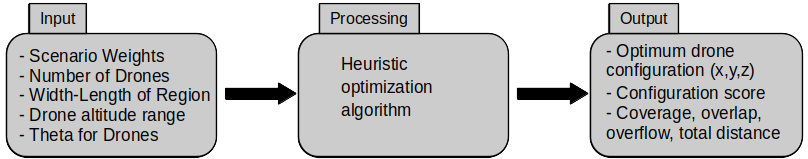
\includegraphics[width=0.9\textwidth]{arch.png}
        \caption{The architecture of the proposed framework.}
        \label{fig:arch1}
    \end{figure}
    %
    %
  
  
   Example Table~\ref{tab:app-type1}.
    %
    %
    %
    \renewcommand{\arraystretch}{1.25}%
    \begin{table}[H]
        \begin{center}
            \caption{Application cases and proposed set of weights.}
            \label{tab:app-type1}
            \begin{adjustbox}{max width=\textwidth}
                \begin{tabular}{| >{}m{7cm} || >{\centering}m{1cm} | >{\centering}m{1cm} | >{\centering}m{1cm} | >{\centering}m{1cm} |}
                    \hline
                    \rowcolor{lightgray}
                    %\textbf{Application type} & \textbf{Coverage\\(\% of Region)} & \textbf{Overlap\\(\% of Covered Region)} & \textbf{Overflow\\(\% of Covered Region)} & \textbf{Mean total distance\\(\% of difference from maximum distance from VBS)} \tabularnewline
                    \textbf{Application type (Scenario)} & $\bm{W_{c}}$ & $\bm{W_{l}}$ & $\bm{W_{f}}$ & $\bm{W_{d}}$ \tabularnewline
                    \hline \hline
                    \cellcolor{lightgray}S1: Max coverage with no compromise                        & +   & 0   & 0  & 0 \tabularnewline \hline
                    \cellcolor{lightgray}S2: Max coverage with only overlap/overflow penalty    & +   & -   & -  & 0 \tabularnewline \hline
                    \cellcolor{lightgray}S3: Max coverage with overlap/overflow penalty and min total distance of drones from VBS   & +   & -   & -  & + \tabularnewline \hline
                    \cellcolor{lightgray}S4: Max coverage with only min total distance of drones from VBS   & +   & 0   & 0  & + \tabularnewline \hline
                    % \cellcolor{lightgray}Total distance is more important than coverage            & +H/L  & -H/L  & -H/L & +H \tabularnewline \hline
                \end{tabular}
                %\\[1.0] %You can adjust how far below the table the text should appear
            \end{adjustbox}
        \end{center}
    \end{table}
    \renewcommand{\arraystretch}{1}%
    %
    %
    %
  
  Example Algorithm~\ref{coverage-algo2}.
    %
    %
    %\algrenewcommand\algorithmicindent{0.5em}%
    
    \begin{algorithm}[H]
        \SetAlgoLined
        \SetKwInOut{KwInput}{Input}\SetKwInOut{KwOutput}{Output}
        \KwInput{Optimisation Parameters: User supplied}
        \KwInput{Region Polygon: User selected on map}
        \KwInput{BS Positions: User selected on map, out of the region polygon}
        \BlankLine
        \KwOutput{Drone positions and the tessellated region polygon}
        \BlankLine
        \textbf{Estimation of VBS (special drones) positions:}\;
        The closest points on the region polygon edges to BS positions are chosen as VBS positions\;
        VBSs are kept at "medium" altitude\;
        \BlankLine
        \textbf{Voronoi Tesselation:}\;
        The VBS points are chosen as "site" points for the tesselation\;
        Weighted/Normal tesselation is carried out dividing region into sub-regions\;
        Number of drones are distributed according to the area of each sub-regions\;
        \BlankLine
        \textbf{Initial Solution:}\;
        Drones are placed hexagonally in the sub-regions\;
        "Extra" (out of hexagonal positions) drones are placed randomly\;
        All drones in the same sub-region are at the same altitude\;
        Initial solution is shown on the map\;
        \BlankLine
        \textbf{Optimum Solution:}\;
        Heuristic evolutionary optimisation tries to improve the supplied initial solution\;
        Optimisation according to the "weights" is carried out for each sub-region\;
        Optimal solution is shown on the map\;
        \BlankLine
        \Return Optimum Drone positions and the tessellated region polygon
        \caption{The proposed "optimum region coverage" algorithm in pseudo code.}\label{coverage-algo2}
    \end{algorithm}
    %%%%%%%%%%%%%%%%%%%%%%%%%%%%%%%%%%%%%%%%%%%%%%%%%%%%%%%%%%%%%%%%%%%%%%%%%%%%%%%%%%%%%%%%%
    
    \section{Motivation}
  
    
    %%%%%%%%%%%%%%%%%%%%%%%%%%%%%%%%%%%%%%%%%%%%%%%%%%%%%%%%%%%%%%%%%%%%%%%%%%%%%%%%%%%%%%%%%
    \section{Objectives}
     
    %%%%%%%%%%%%%%%%%%%%%%%%%%%%%%%%%%%%%%%%%%%%%%%%%%%%%%%%%%%%%%%%%%%%%%%%%%%%%%%%%%%%%%%%%
    \section{Contributions and Impacts of the Thesis}
    
    
    
    %%%%%%%%%%%%%%%%%%%%%%%%%%%%%%%%%%%%%%%%%%%%%%%%%%%%%%%%%%%%%%%%%%%%%%%%%%%%%%%%%%%%%%%%%
    \section{Structure of the Thesis}
    %%%%%%%%%%%%%%%%%%%%%%%%%%%%%%%%%%%%%%%%%%%%%%%%%%%%%%%%%%%%%%%%%%%%%%%%%%%%%%%%%%%%%%%%%
    
    \chapter{Ch1}
   
    %%%%%%%%%%%%%%%%%%%%%%%%%%%%%%%%%%%%%%%%%%%%%%%%%%%%%%%%%%%%%%%%%%%%%%%%%%%%%%%%%%%%%%%%%
    \section{Ch1Sec1}
    \label{ch1s10}
    %%%%%%%%%%%%%%%%%%%%%%%%%%%%%%%%%%%%%%%%%%%%%%%%%%%%%%%%%%%%%%%%%%%%%%%%%%%%%%%%%%%%%%%%%
    \subsection{Ch1Sec1SSec1}
     \textsc{Lorem ipsum dolor} sit amet, consectetur adipisci elit, sed do eiusmod tempor incidunt ut labore et dolore magna aliqua. Ut enim ad minim veniam, quis nostrum exercitationem ullamco laboriosam, nisi ut aliquid ex ea commodi consequatur. Duis aute irure reprehenderit in voluptate velit esse cillum dolore eu fugiat nulla pariatur. Excepteur sint obcaecat cupiditat non proident, sunt in culpa qui officia deserunt mollit anim id est laborum.
     
     
     
     
    
    %%%%%%%%%%%%%%%%%%%%%%%%%%%%%%%%%%%%%%%%%%%%%%%%%%%%%%%%%%%%%%%%%%%%%%%%%%%%%%%%%%%%%%%%%%%%%%%%%%%%%%%%%%%%%%%%%%%%%%%%%%%%%%%%%%%%%%%%%%%%%%%%%%%%%%%%
    \chapter{Conclusions}\label{chap:conc}
   
    
    \textsc{Lorem ipsum dolor} sit amet, consectetur adipisci elit, sed do eiusmod tempor incidunt ut labore et dolore magna aliqua. Ut enim ad minim veniam, quis nostrum exercitationem ullamco laboriosam, nisi ut aliquid ex ea commodi consequatur. Duis aute irure reprehenderit in voluptate velit esse cillum dolore eu fugiat nulla pariatur. Excepteur sint obcaecat cupiditat non proident, sunt in culpa qui officia deserunt mollit anim id est laborum.
    
    %%%%%%%%%%%%%%%%%%%%%%%%%%%%%%%%%%%%%%%%%%%%%%%%%%%%%%%%%%%%%%%%%%%%%%%%%%%%%%%%%%%%%%%%%%%%%%%%%%%%%%%%%%%%%%%%%%%%%%%%%%%%%%%%%%%%%%%%%%%%%%%%%%%%%%%%
    %\appendix
    %\input{schema_elettrico}
    %\input{Appendix1}
    %\input{Appendix2}
    %%%%%%%%%%%%%%%%%%%%%%%%%%%%%%%%%%%%%%%%%%%%%%%%%%%%%%%%%%%%%%%%%%%%%%%%%%%%%%%%%%%%%%%%%%%%%%%%%%%%%%%%%%%%%%%%%%%%%%%%%%%%%%%%%%%%%%%%%%%%%%%%%%%%%%%%
    
    
    
    %%%%%%%%%%%%%%%%%%%%%%%%%%%%%%%%%%%%%%%%%%%%%%%%%%%%%%%%%%%%%%%%%%%%%%%%%%%%%%%%%%%%%%%%%%%%%%%%%%%%%%%%%%%%%%%%%%%%%%%%%%%%%%%%%%%%%%%%%%%%%%%%%%%%%%%%%%%%%%%%
    % \cleardoublepage
    % 
    % \phantomsection
    % 
    % \addcontentsline{toc}{chapter}{Bibliography}
    
    \nocite{*} 
    \cleardoublepage
    \phantomsection
    \addcontentsline{toc}{chapter}{References}
    \bibliography{tesi} %rename to your .bib file
    
    %%%%%%%%%%%%%%%%%%%%%%%%%%%%%%%%%%%%%%%%%%%%%%%%%%%%%%%%%%%%%%%%%%%%%%%%%%%%%%%%%%%%%%%%%%%%%%%%%%%%%%%%%%%%%%%%%%%%%%%%%%%%%%%%%%%%%%%%%%%%%%%%%%%%%%%%%%%%%%%%
    
    
    
    
    %\printbibliography
    
    \printindex
    
    
    %%%%%%%%%%%%%%%%%%%%%%%%%%%%%%%%%%%%%%%%%%%%%%%%%%%%%%%%%%%%%%%%%%%%%%%%%%%%%%%%%%%%%%%%%
    %\chapter*{Ringraziamenti}
    %%%%%%%%%%%%%%%%%%%%%%%%%%%%%%%%%%%%%%%%%%%%%%%%%%%%%%%%%%%%%%%%%%%%%%%%%%%%%%%%%%%%%%%%%
    %Ringrazio...
    %%%%%%%%%%%%%%%%%%%%%%%%%%%%%%%%%%%%%%%%%%%%%%%%%%%%%%%%%%%%%%%%%%%%%%%%%%%%%%%%%%%%%%%%%
    
    
\end{document}
